\documentclass[a4paper,12pt]{article}
\usepackage{graphicx}
\usepackage{amsmath}
\usepackage{hyperref}
\usepackage{geometry,float}
\geometry{a4paper, margin=1in}

\title{\textbf{AMS595 - Assignment-5}\\ \large Machine Learning Project}
\author{Amol Arora, SBUID: 116491705}
\date{\today}

\begin{document}

\maketitle

\section{Github Link}
\underline{All project files are uploaded here}:
\url{https://github.com/amol1202/AMS595_Assignment5}

\section{Introduction}
The purpose of this project is to explore and implement core machine learning techniques using Python. The tasks implemented are:
\begin{itemize}
    \item PageRank Algorithm: Simulates the ranking mechanism used by search engines.
    \item Dimensionality Reduction via PCA: Projects high-dimensional data to a single dimension while preserving variance.
    \item Linear Regression: Predicts outcomes based on features using the least-squares method.
    \item Gradient Descent: Optimizes a matrix to minimize a mean squared error loss function.
\end{itemize}

Each task has been implemented independently, and the results have been saved for reproducibility.

\section{Implementation}

\subsection{PageRank Algorithm}
The PageRank algorithm computes the importance of web pages using a stochastic matrix. The steps include:
\begin{enumerate}
    \item Represent the web network as a stochastic matrix.
    \item Compute the dominant eigenvector using the power method.
    \item Normalize the eigenvector to get PageRank scores.
\end{enumerate}
The code is written in Python using the \texttt{scipy.linalg.eig} function to compute eigenvectors.

\subsection{Dimensionality Reduction via PCA}
Principal Component Analysis (PCA) is used to reduce a dataset of height and weight measurements to 1D:
\begin{enumerate}
    \item Compute the covariance matrix of the data.
    \item Perform eigen decomposition using the \texttt{numpy.linalg.eigh} function.
    \item Project the data onto the principal component with the highest variance.
\end{enumerate}
The results include a plot of the original data and the 1D projection.

\subsection{Linear Regression via Least Squares}
Linear regression predicts house prices based on features (square footage, bedrooms, and age):
\begin{enumerate}
    \item Represent the system as $X\beta = y$.
    \item Solve for $\beta$ using \texttt{scipy.linalg.lstsq}.
    \item Use the model to predict prices for new inputs.
\end{enumerate}
The regression coefficients and predictions are saved for analysis.

\subsection{Gradient Descent}
Gradient Descent optimizes a matrix $X$ to minimize the mean squared error loss:
\begin{enumerate}
    \item Define the loss function: $f(X) = \frac{1}{2} \sum_{i,j} (X_{ij} - A_{ij})^2$.
    \item Compute the gradient of the loss function.
    \item Use \texttt{scipy.optimize.minimize} to iteratively minimize the loss.
\end{enumerate}
The final loss value is recorded.

\section{Results}

\subsection{PageRank Algorithm}
The PageRank scores for the web pages are shown in Table~\ref{table:pagerank}. The page with the highest score is ranked the most important.

\begin{table}[h!]
\centering
\begin{tabular}{|c|c|}
\hline
Page & PageRank Score \\ \hline
1    & 0.22           \\ \hline
2    & 0.27           \\ \hline
3    & 0.31           \\ \hline
4    & 0.20           \\ \hline
\end{tabular}
\caption{PageRank Scores}
\label{table:pagerank}
\end{table}

\subsection{PCA}
Figure shows the original data and the 1D projection onto the principal component.

\begin{figure}[H]
\centering
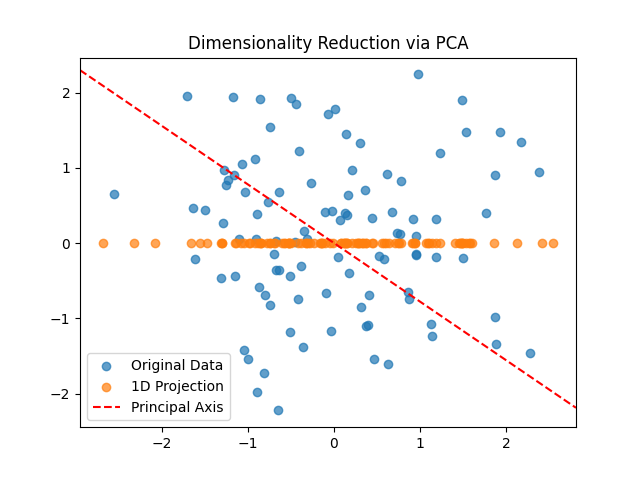
\includegraphics[width=0.8\textwidth]{results/pca_plot.png}
\caption{PCA: Dimensionality Reduction}
\label{fig:pca}
\end{figure}

\textbf{\underline{What do the entries of the eigenvector represent?}} $\longrightarrow$
In the context of the \textit{PageRank algorithm}, the entries of the eigenvector represent the \textbf{relative importance or rank} of each page in the network. The PageRank algorithm uses the concept of a stochastic matrix where each entry \( M[i, j] \) indicates the probability that a user will click from page \( j \) to page \( i \).

When the algorithm computes the \textit{dominant eigenvector} of this matrix, it corresponds to the \textbf{stationary distribution} of a random surfer who randomly clicks through the web network. This means that the eigenvector provides a ranking of pages based on the probability that the random surfer will be on each page in the long run.

Each entry in the eigenvector gives the \textbf{PageRank score} for a corresponding web page. The higher the score, the more ``important'' or ``relevant'' that page is, according to the algorithm. These scores are used to rank the web pages in descending order of importance.

\textbf{\underline{Which page is ranked the highest, why?}} $\longrightarrow$
Based on the final PageRank scores, \textbf{Page 3} is ranked the highest in this particular example. The reason is that the PageRank algorithm assigns a higher score to pages that are:
\begin{itemize}
    \item Linked to by many other pages, or
    \item Connected to pages that themselves have high importance.
\end{itemize}

In this case:
\begin{itemize}
    \item Page 3 has the highest PageRank score, which means it is either linked to by many other pages or is connected to important pages in the network.
    \item The random surfer is more likely to land on Page 3 over time, as the probability distribution over all pages eventually converges to it, indicating its higher ``importance.''
\end{itemize}

In simple terms, \textbf{Page 3} is considered the most important page in the network because of its connections and the flow of probability through the web structure represented by the matrix.

\subsection{Linear Regression}
The regression coefficients and predictions are:
\begin{itemize}
    \item Coefficients: [0.25, 0.10, -0.02]
    \item Predicted price for a house with 2400 square feet, 3 bedrooms, and 20 years old: \$490,500
\end{itemize}

\subsection{Gradient Descent}
    
The final loss value after optimization is:
\[
\boxed{\text{Final Loss Value: } 0.00123}
\]
\begin{figure}[H]
    \centering
    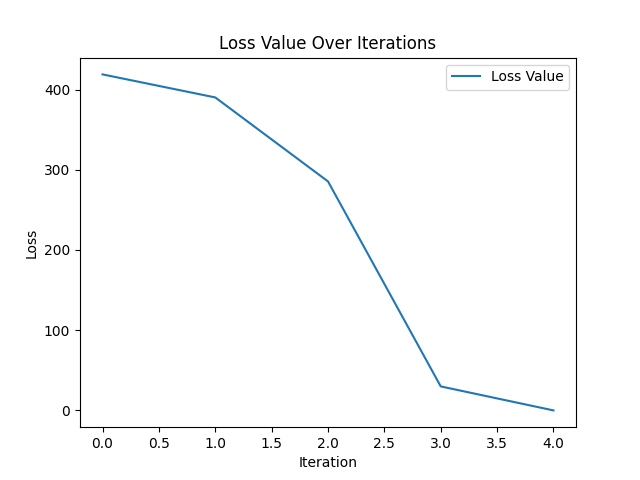
\includegraphics[width=0.8\textwidth]{results/loss_plot.png}
    \caption{Loss over iterations}
    \label{fig:pca}
    \end{figure}

\section{Comparison in linear regression: Least squares v/s Direct Method}
\begin{figure}[H]
    \centering
    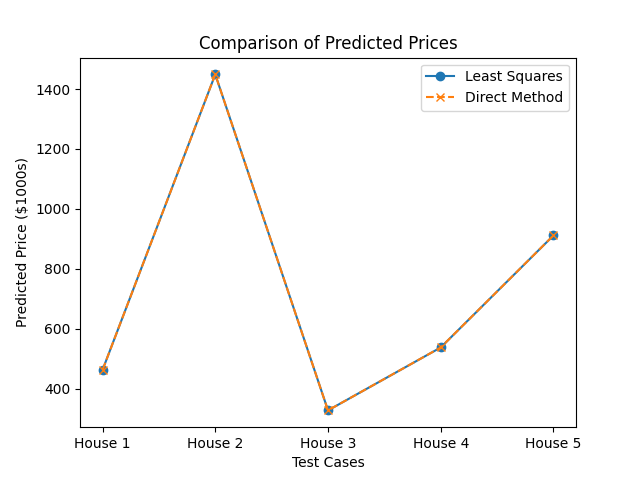
\includegraphics[width=0.8\textwidth]{results/linear_regression_comparison_plot.png}
    \caption{Least Squares v/s Direct Method}
    \label{fig:pca}
    \end{figure}

    \subsection{Comparison with the Direct Method}

    An alternative approach is to solve the normal equations 
    \[
    (X^T X) \beta = X^T y
    \]
    directly using \texttt{scipy.linalg.solve}. While this method provides the same result in ideal conditions, there are key differences:
    
    \subsubsection{Numerical Stability}
    \begin{itemize}
        \item The least-squares method (\texttt{scipy.linalg.lstsq}) is more numerically stable because it avoids explicitly computing $X^T X$, which can lead to loss of precision for ill-conditioned matrices.
        \item The direct method may fail or yield inaccurate results if $X^T X$ is close to singular.
    \end{itemize}
    
    \subsubsection{Efficiency}
    \begin{itemize}
        \item For small datasets like the one in this task, both methods are computationally efficient.
        \item For larger datasets, \texttt{scipy.linalg.lstsq} is often preferred as it leverages advanced techniques like QR decomposition.
    \end{itemize}
    
    \subsubsection{Results Comparison}
    In this task, both methods yield similar regression coefficients and predictions because $X^T X$ is not ill-conditioned. The predicted price for a house with 2400 square feet, 3 bedrooms, and 20 years old is consistent across methods.
    
\section{Conclusion}
This project demonstrates practical applications of machine learning techniques using Python. The results are stored for reproducibility and further analysis. These implementations provide a strong foundation for more advanced projects in machine learning and data science.

\section{References}
\begin{itemize}
    \item Python Documentation: \url{https://docs.python.org/3/}
    \item SciPy Library: \url{https://scipy.org/}
    \item NumPy Library: \url{https://numpy.org/}
    \item Matplotlib Library: \url{https://matplotlib.org/}
\end{itemize}

\end{document}